\documentclass{article}

% packages
\usepackage{amsmath, amsthm, thmtools, amsfonts, amssymb, luacode, catchfile, tikzducks, hyperref, ifthen}
\ifcsname c@kobocompile\endcsname
	\usepackage[a5paper, total={1072pt, 1448pt}, margin=10pt, includeheadfoot]{geometry} % set page margins
\else
	\usepackage[a4paper, margin=50pt, includeheadfoot]{geometry}
\fi
\usepackage[shortlabels]{enumitem}
\usepackage[skip=3pt, indent=0pt]{parskip}

% language
\usepackage[bidi=basic, layout=tabular, provide=*]{babel}
\ifcsname c@english\endcsname
	\babelprovide[main, import]{english}
\else
	\babelprovide[main, import]{hebrew}
	\babelprovide{rl}
\fi
%\babelfont{rm}{Libertinus Serif}
\babelfont{rm}[Renderer=Harfbuzz]{Libertinus Serif}
\babelfont{sf}{Libertinus Sans}
\babelfont{tt}{Libertinus Mono}

% style
\AddToHook{cmd/section/before}{\clearpage}	% Add line break before section
\linespread{1.3}
\setcounter{secnumdepth}{0}		% Remove default number tags from sections, this won't do well with theorems
\AtBeginDocument{\setlength{\belowdisplayskip}{3pt}}
\AtBeginDocument{\setlength{\abovedisplayskip}{3pt}}
\graphicspath{ {../images/} }

% operators
\DeclareMathOperator\cis{cis}
\DeclareMathOperator\Sp{Sp}
\DeclareMathOperator\tr{tr}
\DeclareMathOperator\im{Im}
\DeclareMathOperator\re{Re}
\DeclareMathOperator\diag{diag}
\DeclareMathOperator*\lowlim{\underline{lim}}
\DeclareMathOperator*\uplim{\overline{lim}}
\DeclareMathOperator\rng{rng}
\DeclareMathOperator\Sym{Sym}
\DeclareMathOperator\Arg{Arg}
\DeclareMathOperator\Log{Log}
\DeclareMathOperator\dom{dom}
\DeclareMathOperator\supp{Supp}
\DeclareMathOperator\var{Var}
\DeclareMathOperator\cov{Cov}

% commands
%\renewcommand\qedsymbol{\textbf{מש''ל}}
%\renewcommand\qedsymbol{\fbox{\emoji{lizard}}}
\newcommand{\Aa}[0]{\mathcal{A}}
\newcommand{\Bb}[0]{\mathcal{B}}
\newcommand{\CC}[0]{\mathbb{C}}
\newcommand{\Cc}[0]{\mathcal{C}}
\newcommand{\EE}[0]{\mathbb{E}}
\newcommand{\FF}[0]{\mathbb{F}}
\newcommand{\Ff}[0]{\mathcal{F}}
\newcommand{\Ii}[0]{\mathcal{I}}
\newcommand{\Gg}[0]{\mathcal{G}}
\newcommand{\Ll}[0]{\mathcal{L}}
\newcommand{\Mm}[0]{\mathcal{M}}
\newcommand{\NN}[0]{\mathbb{N}}
\newcommand{\Nn}[0]{\mathcal{N}}
\newcommand{\PP}[0]{\mathbb{P}}
\newcommand{\Pp}[0]{\mathcal{P}}
\newcommand{\QQ}[0]{\mathbb{Q}}
\newcommand{\RR}[0]{\mathbb{R}}
\newcommand{\Rr}[0]{\mathcal{R}}
\newcommand{\Ss}[0]{\mathcal{S}}
\newcommand{\TT}[0]{\mathbb{T}}
\newcommand{\Uu}[0]{\mathcal{U}}
\newcommand{\Vv}[0]{\mathcal{V}}
\newcommand{\Ww}[0]{\mathcal{W}}
\newcommand{\ZZ}[0]{\mathbb{Z}}
\newcommand{\acts}[0]{\circlearrowright}
\newcommand{\explain}[2] {
	\begin{flalign*}
		 && \text{#2} && \text{#1}
	\end{flalign*}
}
\newcommand{\maketitleprint}[0]{ \begin{center}
	%\begin{tikzpicture}[scale=3]
	%	\duck[graduate=gray!20!black, tassel=red!70!black]
	%\end{tikzpicture}	
	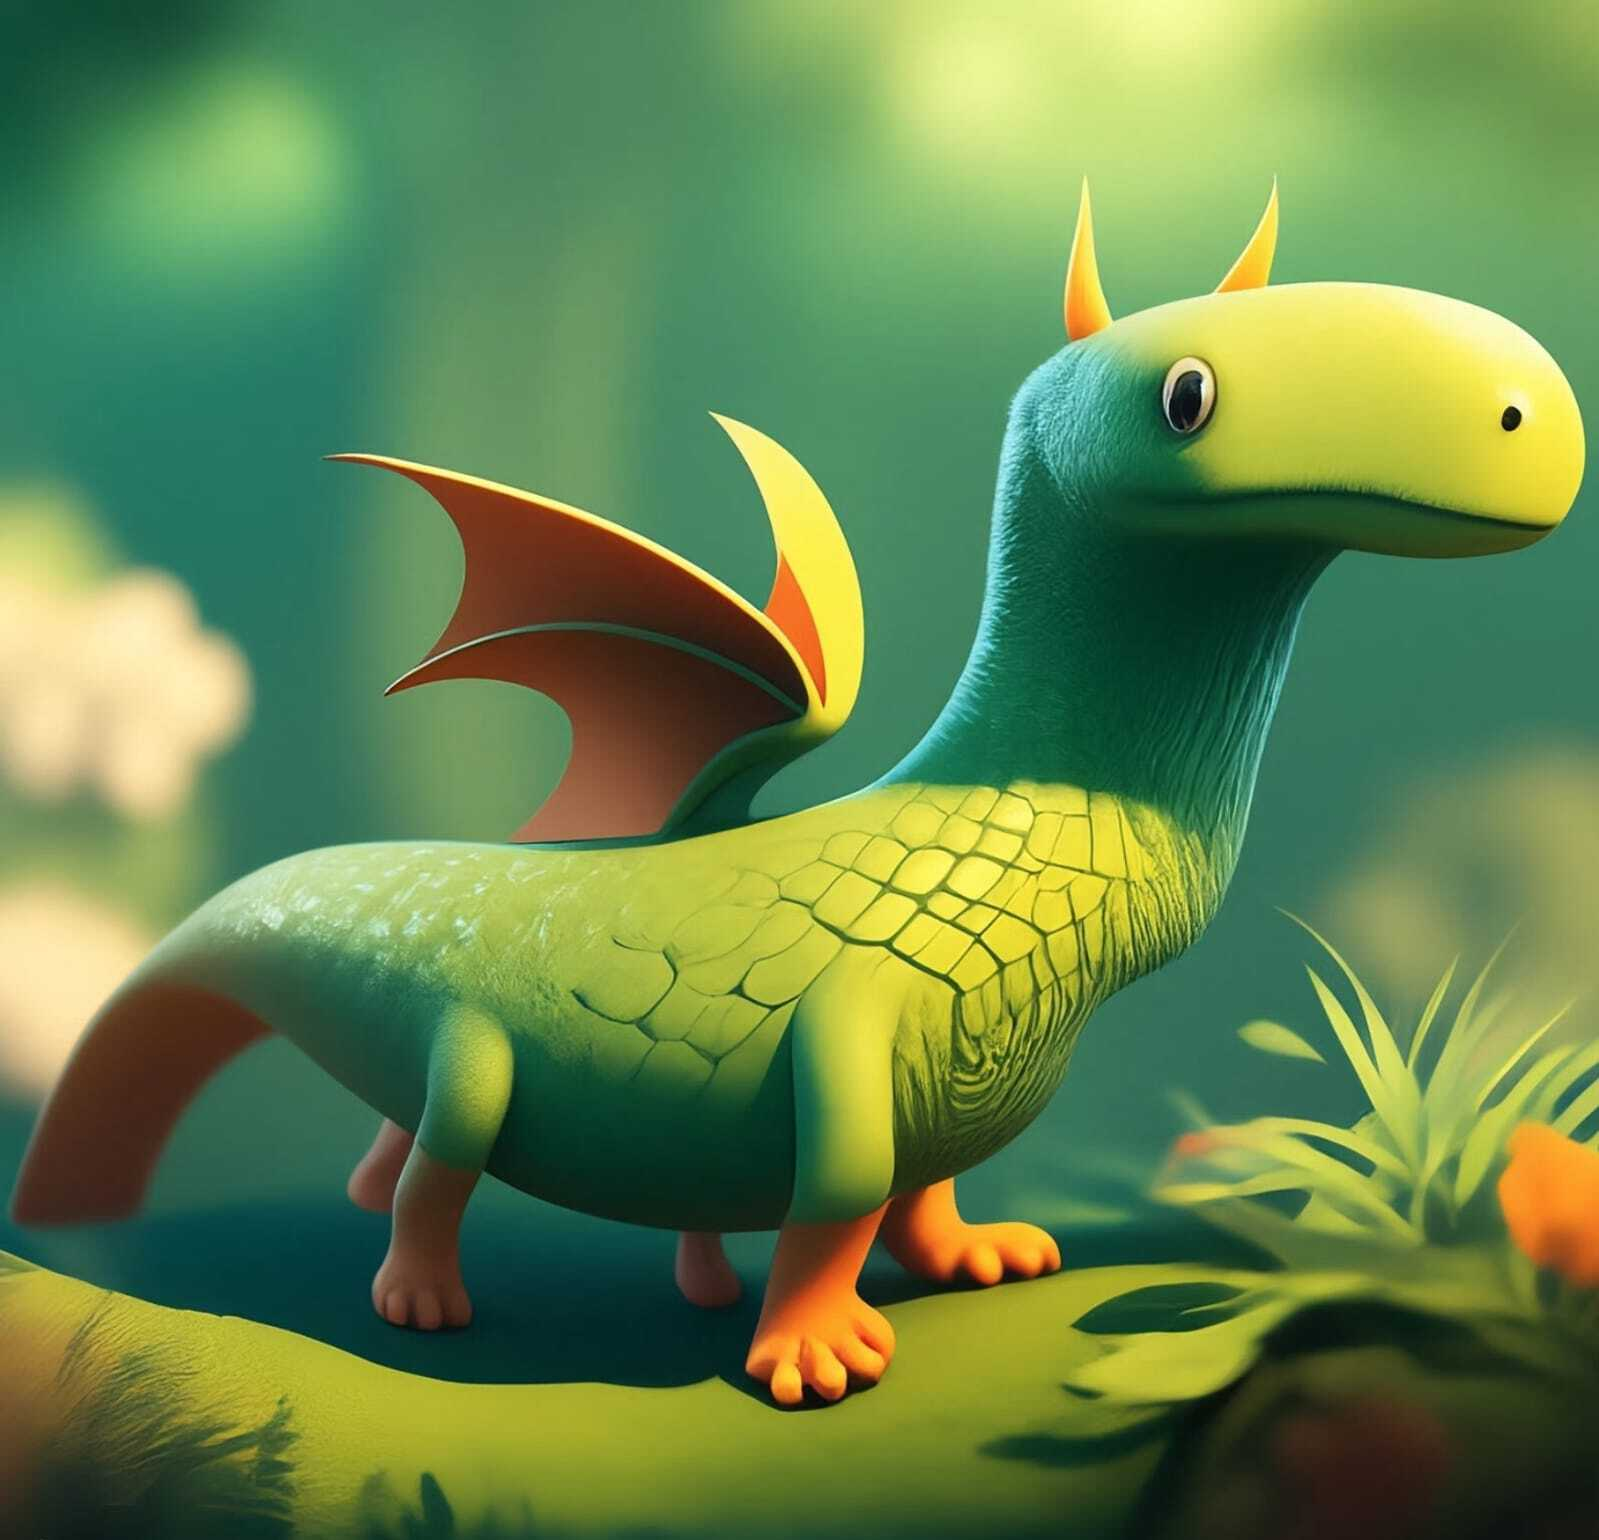
\includegraphics[width=6cm]{cover}
\end{center}
}

% theorem commands
\newtheoremstyle{c_remark}
	{}	% Space above
	{}	% Space below
	{}% Body font
	{}	% Indent amount
	{\bfseries}	% Theorem head font
	{}	% Punctuation after theorem head
	{.5em}	% Space after theorem head
	{\thmname{#1}\thmnumber{ #2}\thmnote{ \normalfont{\text{(#3)}}}}	% head content
\newtheoremstyle{c_definition}
	{3pt}	% Space above
	{3pt}	% Space below
	{}% Body font
	{}	% Indent amount
	{\bfseries}	% Theorem head font
	{}	% Punctuation after theorem head
	{.5em}	% Space after theorem head
	{\thmname{#1}\thmnumber{ #2}\thmnote{ \normalfont{\text{(#3)}}}}	% head content
\newtheoremstyle{c_plain}
	{3pt}	% Space above
	{3pt}	% Space below
	{\itshape}% Body font
	{}	% Indent amount
	{\bfseries}	% Theorem head font
	{}	% Punctuation after theorem head
	{.5em}	% Space after theorem head
	{\thmname{#1}\thmnumber{ #2}\thmnote{ \text{(#3)}}}	% head content

\ifcsname c@english\endcsname
	\theoremstyle{plain}
	\newtheorem{theorem}{Theorem}[section]
	\newtheorem{lemma}[theorem]{Lemma}
	\newtheorem{proposition}[theorem]{Proposition}
	\newtheorem*{proposition*}{Proposition}
	%\newtheorem{corollary}[theorem]{אין חלופה עברית}

	\theoremstyle{definition}
	\newtheorem{definition}[theorem]{Definition}
	\newtheorem*{definition*}{Definition}
	\newtheorem{example}{Example}[section]
	\newtheorem{exercise}{Exercise}[section]

	\theoremstyle{remark}
	\newtheorem*{remark}{Remark}
	\newtheorem*{solution}{Solution}
	\newtheorem{conclusion}[theorem]{Conclusion}
	\newtheorem{notation}[theorem]{Notation}
\else
	\theoremstyle{c_plain}
	\newtheorem{theorem}{משפט}[section]
	\newtheorem{lemma}[theorem]{למה}
	\newtheorem{proposition}[theorem]{טענה}
	\newtheorem*{proposition*}{טענה}
	%\newtheorem{corollary}[theorem]{אין חלופה עברית}

	\theoremstyle{c_definition}
	\newtheorem{definition}[theorem]{הגדרה}
	\newtheorem*{definition*}{הגדרה}
	\newtheorem{example}{דוגמה}[section]
	\newtheorem{exercise}{תרגיל}[section]

	\theoremstyle{c_remark}
	\newtheorem*{remark}{הערה}
	\newtheorem*{solution}{פתרון}
	\newtheorem{conclusion}[theorem]{מסקנה}
	\newtheorem{notation}[theorem]{סימון}
\fi

% Questions related commands
\newcounter{question}
\setcounter{question}{1}
\newcounter{sub_question}
\setcounter{sub_question}{1}

\ifcsname c@english\endcsname
	\newcommand{\question}[1][0]{
		\ifthenelse{#1 = 0}{}{\setcounter{question}{#1}}
		\section{Question \arabic{question}}
		\addtocounter{question}{1}
		\setcounter{sub_question}{1}
	}

	\newcommand{\subquestion}[1][0]{
		\ifthenelse{#1 = 0}{}{\setcounter{sub_question}{#1}}
		\subsection{Part \alph{sub_question}}
		\addtocounter{sub_question}{1}
	}
\else
	\newcommand{\question}[1][0]{
		\ifthenelse{#1 = 0}{}{\setcounter{question}{#1}}
		\section{שאלה \arabic{question}}
		\addtocounter{question}{1}
		\setcounter{sub_question}{1}
	}

	\newcommand{\subquestion}[1][0]{
		\ifthenelse{#1 = 0}{}{\setcounter{sub_question}{#1}}
		\subsection{סעיף \localecounter{letters.gershayim}{sub_question}}
		\addtocounter{sub_question}{1}
	}
\fi

% import lua and start of document
\directlua{common = require ('../common')}

\GetEnv{AUTHOR}

% headers
\author{\AUTHOR}
\date\today

\title{פתרון מטלה 04 --- אנליזה על יריעות, 80426}

\DeclareMathOperator{\vol}{vol}

\begin{document}
\maketitle
\maketitleprint{}

\question{}
תהי $U = {(0, 1)}^2$ ותהי ההעתקה $\varphi : U \to \RR^3$ המוגדרת על־ידי $\varphi(x, y) = (x, y, e^{x + y})$. \\
נסמן $X = \im \varphi$ וב־$d \vol_2$ את אלמנט הנפח, נחשב את,
\[
	\int_X \sqrt{2z^2 + 1}\ d\vol_2
\]
\begin{solution}
	אם נסמן $f(x, y, z) = \sqrt{2z^2 + 1}$ אז נקבל שמתקיים,
	\[
		\int_X \sqrt{2z^2 + 1}\ d\vol_2
		= \int_U f(\varphi(u)) V(D \varphi \mid_u)\ du
	\]
	נחשב את הנגזרת של $\varphi$,
	\[
		D\varphi
		= \begin{pmatrix}
			1 & 0 \\
			0 & 1 \\
			e^{x + y} & e^{x + y}
		\end{pmatrix} 
	\]
	מתוך כוונה להשתמש בלמה לחישוב $V(D \varphi)$ נחשב,
	\[
		V(D\varphi)
		= \sqrt{{(D\varphi)}^t D \varphi}
		= \sqrt{\begin{vmatrix}
				1 + e^{{(x + y)}^2} & e^{{(x + y)}^2} \\
				e^{{(x + y)}^2} & 1 + e^{{(x + y)}^2}
		\end{vmatrix}}
		= \sqrt{1 + 2e^{{(x + y)}^2}}
	\]
	ולכן נציב,
	\[
		\int_{(0, 1)} \int_{(0, 1)} \sqrt{2 e^{{(x + y)}^2} + 1} \cdot \sqrt{1 + 2 e^{{(x + y)}^2}}\ dx\ dy
		= \int_{(0, 1)} \int_{(0, 1)} 2 e^{{(x + y)}^2} + 1\ dx\ dy
	\]
	ואין לי מושג איך לחשב את זה.
\end{solution}

\question{}
\subquestion{}
תהי פונקציה $f : [a, b] \to (0, \infty)$ גזירה ברציפות, ויהי גוף הסיבוב שלה,
\[
	\Sigma_f
	= \{ (x, y, z) \in \RR^3 \mid z \in [a, b], \sqrt{x^2 + y^2} = f(z) \}
\]
נראה ש־$(\varphi, \Sigma_f)$ היא יריעה דו־מימדית, כאשר,
\[
	\varphi(t, z)
	= (f(z) \cos t, f(z) \sin t, z)
\]
עבור $(t, z) \in [0, 2\pi] \times [a, b] = K$.
\begin{proof}
	נבחין כי הקבוצה עליה $\varphi$ מוגדרת היא קבוצה סגורה (למעשה דיסק סגור), בסתירה להגדרה של יריעה, כשנדבר על היריעה נוכל להתכוון לדיסק הפתוח ובכך לפתור את הבעיה.
	עלינו להראות ש־$\varphi(K) = \Sigma_f$.
	\[
		(x, y, z) = \varphi(t, z)
		\implies \sqrt{x^2 + y^2}
		= \sqrt{f^2(z) \cos^2 t + f^2(z) + f^2(z) \sin^2 t}
		= \sqrt{f^z(z)}
		= f(z)
	\]
	כאשר המהלך האחרון נובע מהעובדה ש־$f$ חיובית לחלוטין.
	נובע ש־$\varphi(K) \subseteq \Sigma_f$.
	תהי $(x, y, z) \in \Sigma_f$, אז נבחר $t = \Arg(x + iy)$ ונקבל מהגדרת הארגומנט ש־$\varphi(t, z) = (x, y, z)$, לכן גם $\varphi(K) \supseteq \Sigma_f$, ונסיק $\varphi(K) = \Sigma_f$ כפי שרצינו.
\end{proof}
נחשב את $\vol_2(\Sigma_f)$.
\begin{solution}
	נחשב את $V(D\varphi)$,
	\[
		D\varphi
		= \begin{pmatrix}
			- f(z) \sin t & f'(z) \cos t \\
			f(z) \cos t & f'(z) \sin t \\
			0 & 1
		\end{pmatrix} 
	\]
	ולכן,
	\begin{align*}
		V(D\varphi)
		& = \sqrt{\begin{vmatrix}
				f^2(z) \sin^2 t + f^2(z) \cos^2 t & -f(z) f'(z) \sin t \cos t + f(z) f'(z) \sin t \cos t \\
				-f(z) f'(z) \sin t \cos t + f(z) f'(z) \sin t \cos t & {(f'(z))}^2 \cos^2 t + {(f'(z))}^2 \sin^2 t + 1
		\end{vmatrix}} \\
		& = \sqrt{\begin{vmatrix}
				f^2(z) & 0 \\
				0 & {(f'(z))}^2 + 1
		\end{vmatrix}}
		= f(z) \sqrt{{(f'(z))}^2 + 1}
	\end{align*}
	מהגדרת הנפח,
	\[
		\vol(\Sigma_f)
		= \int_K V(D \varphi \mid_u)\ du
		= 2\pi \int_a^b f(z) \sqrt{{(f'(z))}^2 + 1}\ dz
	\]
\end{solution}

\subquestion{}
נחשב את,
\[
	\int_{\Sigma_f} x^2 + y^2\ d\vol_2
\]
\begin{solution}
	אנו כבר יודעים את ערך $V(D \varphi)$ ולכן נותר להציב,
	\[
		\int_{\Sigma_f} x^2 + y^2\ d\vol_2
		= \int_K f^2(z) \cdot f(z) \sqrt{{(f'(z))}^2 + 1}\ dz\ dt
		= 2\pi \int_a^b f^3(z) \sqrt{{(f'(z))}^2 + 1}\ dz
	\]
\end{solution}

\question{}
\subquestion{}
נחשב את מרכז המסה של,
\[
	S_+^2
	= \{ (x, y, z) \in \RR^3 \mid x^2 + y^2 + z^2 = 1, z, y, z \ge 0 \}
\]
\begin{solution}
	נתחיל בחישוב השטח של העקומה,
	נגדיר $\varphi(x, y) = (x, y, \sqrt{1 - x^2 - y^2})$,
	נחשב את $D\varphi$,
	\[
		D\varphi
		= \begin{pmatrix}
			1 & 0 \\
			0 & 1 \\
			\frac{-x}{\sqrt{1 - x^2 - y^2}} & \frac{-y}{\sqrt{1 - x^2 - y^2}}
		\end{pmatrix}
	\]
	ובהתאם נקבל שגם,
	\[
		V(D\varphi)
		= \sqrt{{(D\varphi)}^t D\varphi}
		= \sqrt{\begin{vmatrix}
				1 + \frac{x^2}{1 - x^2 - y^2} & \frac{xy}{1 - x^2 - y^2} \\
				\frac{xy}{1 - x^2 - y^2} & 1 + \frac{y^2}{1 - x^2 - y^2}
		\end{vmatrix}}
		= \frac{1}{\sqrt{1 - x^2 - y^2}}
	\]
	השטח מתקבל אם כך על־ידי,
	\[
		\vol_2(S_+^2)
		= \int_0^1 \int_0^{\sqrt{1 - x^2}} \frac{1}{\sqrt{1 - x^2 - y^2}}\ dy\ dx
		= \frac{\pi}{4} \int_0^1 \frac{1}{\sqrt{1 - r^2}} \cdot r\ dr
		= \frac{\pi}{4} \int_{1}^{0} \frac{1}{\sqrt{t}}\ dt
		= \frac{\pi}{4} 2 \sqrt{1}
		= \frac{\pi}{2}
	\]
	מטעמי סימטריה מספיק שנבדוק את אחד מהצירים בלבד, נבחר את ציר ה־$x$.
	אנו יודעים ש־$x_{cm} = \frac{1}{\vol_2(S_+^2)} \int_{S_+^2} x\ d\vol_2$, ולכן,
	\begin{align*}
		x_{cm}
		& = \frac{2}{\pi} \int_0^1 \int_0^{\sqrt{1 - x^2}} \frac{x}{\sqrt{1 - x^2 - y^2}}\ dy\ dx \\
		& = \frac{2}{\pi} \int_{0}^{\frac{\pi}{2}} \int_{0}^{1} r \cdot \frac{r \cos \theta}{\sqrt{1 - r^2}}\ dr\ d\theta \\
		& = \frac{2}{\pi} {\left[ \sin \theta \right]}_{\theta = 0}^{\theta = \frac{\pi}{2}} \cdot \int_0^1 \frac{r^2}{\sqrt{1 - r^2}}\ dr \\
		& = \frac{2}{\pi} \cdot 1 \cdot \frac{\pi}{4} \\
		& = \frac{1}{2}
	\end{align*}
	ולכן מרכז המסה הוא $(\frac{1}{2}, \frac{1}{2}, \frac{1}{2})$.
\end{solution}

\subquestion{}
נראה שאם $M, N \subseteq \RR^n$ יריעות פרמטריות זרות עם אותו מימד,
אז $M \cup N$ היא יריעה פרמטרית כך שמרכז המסה שלה הוא הממוצע המשוכלל,
\[
	\vec{c}_{M \cup N}
	= \frac{\vol(M) \vec{c}_M + \vol(N) \vec{c}_N}{\vol(M) + \vol(N)}
\]
\begin{proof}
	נניח ש־$\varphi_M, \varphi_N$ הפרמטריזציה של היריעות $M, N$ בהתאמה.
	נרצה לבחור פרמטריזציה $\varphi : U \to \RR^d$ כך ש־$\varphi(U) = M \cup N$, אך $\dom \varphi_M, \dom \varphi_N$ לא בהכרח זרות.

	נוכיח אם כן שקיים דיפאומורפיזם $\psi : \RR^d \to {(-1, 1)}^d$.
	נגדיר $\psi_i(x_i) = \frac{2}{\pi} \arctan x_i$ ונקבל מתכונות $\tan$ שאכן $\psi$ פונקציה רציפה, הפיכה וכן מגזירות $\tan$ שהיא דיפאומורפיזם.

	נוכל אם כן להניח ש־$\dom \varphi_M \cap \dom \varphi_N = \emptyset$, שאם לא כן, נוכל לבחור $\psi \circ \varphi_M$ ו־$1^d + \psi \circ \varphi_N$ כאשר $1^d = (1, \ldots, 1)$.

	נסיק שקיימים תחומים זרים $U_M, U_N$ כך ש־$\varphi \restriction U_M = \varphi_M, \varphi \restriction U_N = \varphi_N$.
	בהתאם נוכל לחשב את נפח $N \cup M$,
	\begin{align*}
		\vol_d(M \cup N)
		& = \int_{U_N \uplus U_M} V(D\varphi)\ d\vol_d u \\
		& = \int_{U_N} V(D\varphi)\ d\vol_d + \int_{U_M} V(D\varphi)\ d\vol_d u \\
		& = \int_{U_N} V(D\varphi_N)\ d\vol_d + \int_{U_M} V(D\varphi_M)\ d\vol_d u \\
		& = \vol_d(M) + \vol_d(N)
	\end{align*}
	נעבור לחישוב מרכז המסה $\vec{c}_{M \cup N}$,
	\[
		\vec{c}_{M \cup N}
		= \frac{1}{\vol_d(M \cup N)} \int_{M \uplus N} \vec{u}\ d\vol_d \vec{u}
		= \frac{1}{\vol_d(M \cup N)} \left( \int_{M} \vec{u}\ d\vol_d \vec{u} + \int_{M} \vec{u}\ d\vol_d \vec{u} \right)
		= \frac{\vol(M) \vec{c}_M + \vol(N) \vec{c}_N}{\vol(M) + \vol(N)}
	\]
	כאשר המעבר האחרון נובע ישירות מההגדרה של $\vec{c}_M$ ו־$\vec{c}_N$.
\end{proof}

\subquestion{}
נחשב את מרכז המסה של החרוט הסגור,
\[
	\{ \sqrt{x^2 + y^2} = 1 - z \mid 0 < z < 1 \} \cup \{ x^2 + y^2 \le 1, z = 0 \}
\]
\begin{solution}
	נבחין כי החרוט הסגור אינו אלא יריעה פרמטרית של חרוט פתוח ושל עיגול, שתיהן יריעות ממימד 2 ב־$\RR^3$.
	נסמן את החרוט ב־$M$ ואת העיגול ב־$N$, וכן נבחין שמטעמי סימטריה $\vec{c}_N = 0$, וש־$\vol_2(N) = \pi$.
	נעבור אם כך לחישוב הנפח של $M$.
	נגדיר $\varphi : B_1(0) \to M$ על־ידי $\varphi(x, y) = (x, y, 1 - \sqrt{x^2 + y^2})$.
	נעבור לחישובים הכרחיים עבור חישוב האינטגרל,
	\[
		D\varphi
		= \begin{pmatrix}
			1 & 0 \\
			0 & 1 \\
			-\frac{x}{\sqrt{x^2 + y^2}} & -\frac{y}{\sqrt{x^2 + y^2}}
		\end{pmatrix}
	\]
	וכן,
	\[
		V(D\varphi)
		= \sqrt{\begin{vmatrix}
				1 + \frac{x^2}{x^2 + y^2} & \frac{xy}{x^2 + y^2} \\
				\frac{xy}{x^2 + y^2} & 1 + \frac{y^2}{x^2 + y^2}
		\end{vmatrix}}
		= \sqrt{1 + \frac{x^2 + y^2}{x^2 + y^2}}
		= \sqrt{2}
	\]
	ועתה נעבור לחישוב הנפח,
	\[
		\vol_2(M)
		= \int_{B_1(0)} V(D\varphi \mid_u)\ d\vol_2 u
		= \int_{B_1(0)} \sqrt{2}\ du
		= \sqrt{2} \cdot \pi
	\]
	נחשב את מרכז המסה, נבחין שמטעמי סימטריה $c_M^x = c_M^y = 0$ ועלינו לחשב רק את ציר ה־$z$.
	\[
		c_M^z
		= \frac{1}{\sqrt{2} \pi} \int_M z\ d\vol_2 u
		= \frac{1}{\pi} \int_{B(0, 1)} 1 - \sqrt{x^2 + y^2}\ dx\ dy
		= \frac{1}{\pi} (\pi - \int_{0}^{2 \pi} \int_{0}^{1} r^2\ dr\ d \theta)
		= \frac{1}{\pi} (\pi - 2 \pi \cdot \frac{1}{3})
		= \frac{1}{3}
	\]
	ולבסוף נשתמש בתוצאת סעיף ב' ונקבל,
	\[
		\vec{c}_{M \cup N}
		= \frac{\sqrt{2}\pi \cdot (0, 0, \frac{1}{3}) + \pi (0, 0, 0)}{\sqrt{2}\pi + \pi}
		= \left(0, 0, \frac{\sqrt{2}}{3(\sqrt{2} + 1)}\right)
	\]
\end{solution}

\question{}
תהי $(\varphi, M \subseteq \RR^m)$ ו־$(\psi, N \subseteq \RR^n)$ שתי יריעות פרמטריות.
תהינה $f : M \to \RR$ ו־$g : N \to \RR$ פונקציות רציפות.
נגדיר $h : M \times N \to \RR$ על־ידי $h(x, y) = f(x) g(y)$.
נראה שמתקיים,
\[
	\int_{M \times N} h\ d\vol_{n + m}
	= \left( \int_M f\ d\vol_m \right) \cdot \left( \int_N f\ d\vol_n \right)
\]
\begin{proof}
	נניח ש־$\dom \varphi = U_M, \dom \psi = U_N$.
	נגדיר גם $\sigma : U_M \times U_N \to M \times N$ על־ידי $\sigma(x, y) = (\varphi(x), \psi(y))$.
	נסיק ממכפלת מרחבים מטריים ש־$\sigma$ דיפאומורפיזם ולכן מתקיים, נניח ש־$\RR^{n + m} \ni u = (x, y)$ עבור $x \in \RR^m, y \in \RR^n$.
	\[
		\int_{M \times N} h\ d\vol_{n + m}
		= \int_{U_M \times U_N} h(\sigma(u))\ V(D \sigma \mid_u)\ du
		= \int_{U_M \times U_N} f(\varphi(x)) g(\psi(y))\ V(D \sigma \mid_{(x, y)})\ d(x, y)
	\]
	אילו $V(D \sigma) = V(D \varphi) \cdot V(D \psi)$ אז ממשפט פוביני של אינפי 3 נובע ישירות,
	\begin{align*}
		\int_{U_M \times U_N} f(\varphi(x)) g(\psi(y))\ V(D \sigma \mid_{(x, y)})\ d(x, y)
		& = \int_{U_M} f(\varphi(x))\ V(D \varphi \mid_x)\ dx \cdot \int_{U_N} f(\phi(y))\ V(D \psi \mid_y)\ dy \\
		& = \left( \int_M f\ d\vol_m \right) \cdot \left( \int_N f\ d\vol_n \right)
	\end{align*}
	מלינארית אנו יודעים שדטרמיננטת מטריצות בלוקים שווה למכפלת הדטרמיננטות של הבלוקים כמטריצות, לכן מספיק שנראה שאכן ${(D \sigma)}^t (D \sigma)$ מטריצת בלוקים.
	למעשה, הגדרנו את $\sigma$ כך ש־$\sigma(x, 0) = (\varphi(x), 0)$ ולכן נוכל להסיק שאכן $\frac{\partial \sigma}{\partial y_i} = 0$ לכל $1 \le i \le m$, ונסיק שאכן,
	\[
		V(D \sigma) = V(D \varphi) \cdot V(D \psi)
	\]
	ונסיק שהשוויון אכן קיים.
\end{proof}

\end{document}
